\section{Introduction}
This note describes study of diboson production, WW and WZ,
using the CMS detector~\cite{JINST} in events with a leptonically 
decaying W boson  (W$\to\ell\nu$, $\ell=e,\mu$) and one other 
W or Z boson that decays to $q\bar{q}$.


The sample is dominated by associated production of W boson 
with two or more jets, but also contains diboson events with hadronic 
W or Z decay to two jets (W/Z$\to jj$), 
and small contribution from 
top pair ($\ttbar\to l\nu jj$), single top ($pp\to tq \to \ell\nu jj$),
and QCD multijet events. 
We analyze data sample corresponding to an integrated 
luminosity of 5.0~fb${}^{-1}$.



%%%%%%%%%%%%%%%
\subsection{Diboson production}
The self-interaction of the gauge bosons (W, Z, and photon) 
is a consequence of the non-Abelian gauge symmetry of the Standard Model (SM). 
The gauge boson self-interactions appear as vertices involving three 
gauge bosons, and result in the production of pairs of bosons 
as shown in Figures~\ref{figure:diboson_feynman}-\ref{fig:wz_feynman}. 
This pair production of vector bosons is a very interesting process 
because it allows us to test how they couple to one another, something 
which one cannot do by producing them one at a time. 
The study of diboson production thus directly tests the predicted 
SM couplings. 
Observations of anomalous couplings would be an indication of new physics.
Also, Higgs boson may decay into WW or ZZ pairs, giving rise to the same 
final state as the one that is studied in diboson production. 
In addition, Higgs itself can be produced together with one 
vector boson giving the same final state. 


Diboson production was first seen at the Tevatron proton-antiproton 
collider~\cite{Hobbs:2010yg, CDF-diboson-lvjj-2010}, 
and then studied at LEP II where a  pair of W bosons was created from 
electron-positron annihilation. 
Later still, WZ production was seen at the Tevatron, and finally, more 
recently, ZZ production has also been discovered~\cite{Hobbs:2010yg}.
%%%%%%%
\begin{figure}[h!] {\centering
    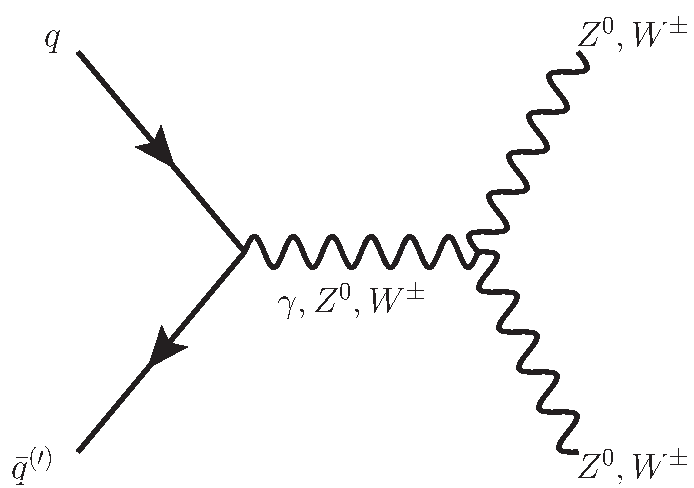
\includegraphics[width=0.5\textwidth]{figs/diboson_generic.pdf}
    \caption{Leading order diagram for WW and ZZ production via
  quark-antiquark annihilation involving the trilinear gauge coupling.}
    \label{figure:diboson_feynman}}
\end{figure}
%%%%%%%
%%%%%%%
\begin{figure}[h!] {\centering
\unitlength=0.33\linewidth
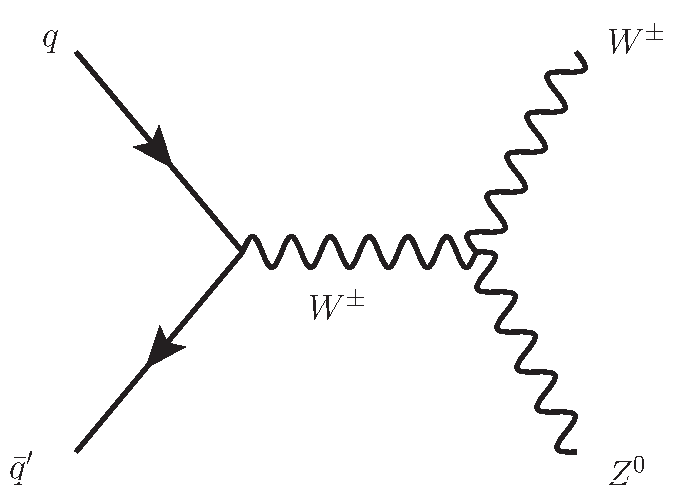
\includegraphics[width=0.48\textwidth]{figs/wz_schannel.pdf}
\put(-0.80,0.0){(a)} 
\unitlength=0.33\linewidth
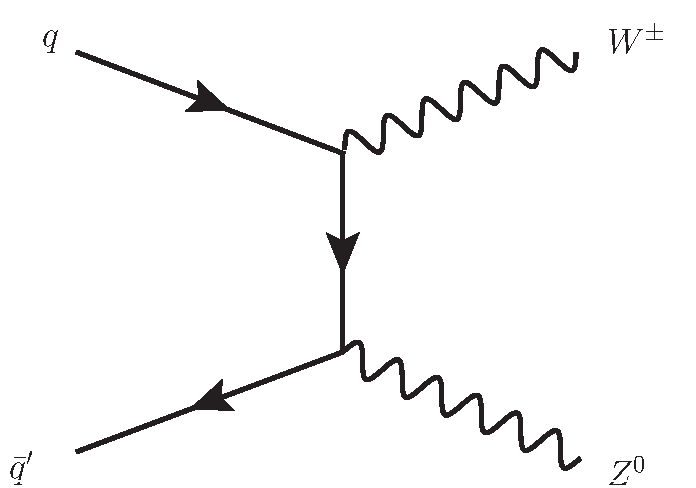
\includegraphics[width=0.48\textwidth]{figs/wz_tchannel.pdf}
\put(-0.80,0.0){(b)} 
\caption{Leading order (a) $s$-channel and (b) $t$-channel diagrams for
  WZ production at the LHC. The $t$-channel diagram for WW production 
  is also the same as (b) except that Z is replaced by W in the 
  outgoing leg.} 
\label{fig:wz_feynman}}
\end{figure}
%%%%%%%
%%%%%%%%%%%%%%%
\subsection{Why study diboson production in \texorpdfstring{$\ell\nu jj$}{l-nu-jj} decay mode ?}
The advantage of reconstructing WW+WZ in $\ell\nu jj$ decay mode over 
the purely leptonic channels is the larger branching fraction to jets, 
at the expense of larger backgrounds, mainly from W+jets.
Compared to the pure WW leptonic diboson decay the semi-leptonic 
process has the ability to  provide a direct handle on the boson transverse 
momentum. 
The sensitivity to very high boson $p_T$ makes this process particularly 
useful as a probe of the gauge structure (symmetries) at high energies 
where we anticipate new physics.
Also, it is possible to reconstruct the 4-body invariant mass of the 
semi-leptonic decay particles ($m_{\ell\nu jj}$) if one solves the 
quadratic equation to extract $p_z$ of the neutrino.


Electron or muon from the leptonic decay of the W is used to trigger 
the event (along with requirement on $\met$).
The shape of dijet mass spectrum is used to discriminate the hadronic 
$W/Z\to jj$  decay from the W+jets, $\ttbar$, single top, and QCD multijet 
processes.


On the flip side, this channel is beset by a large background from 
single $W$ boson produced in association with quarks and/or gluons.

%%%%%%%%%%%%%%%
\subsection{We cannot distinguish between hadronic W and Z}
The $W$ and $Z$ masses differ by about 10 GeV. However, the dijet mass resolution 
of the CMS detector near 80--100 GeV is about 12\%, hence insufficient to distinguish between W$\to jj$ 
and Z$\to jj$ decay processes. 
Therefore, our signal contains a mixture of WW and WZ events.  

%%%%%%%%%%%%%%%
\subsection{Triple gauge couplings}
Production of W boson pairs involves both WW$\gamma$ and WWZ couplings.
Production of WZ involves the WWZ triple gauge coupling (TGC).
The study of WZ production allows one to search for anomalous WWZ coupling 
independent of the WW$\gamma$ coupling in contrast to WW production.
One can potentially 
isolate the WZ contribution by studying diboson production 
in final states containing a lepton, neutrino, and a pair of $b$-quark jets. 
However, the small size of the dataset with two b-jets doesn't allow 
this in the first round of analysis presented here.
%%%%%%%%%%%%%%%%%
%%\subsection{Connection with Higgs}
%%The Higgs mechanism was conceived to give mass to the $W$ and 
%%$Z$ bosons and break the electroweak gauge symmetry. 
%%The mechanism predicts a Higgs boson particle that interacts with other 
%%particles with a strength proportional to their mass.
%%Since the $W$ and $Z$ bosons are very massive, the Higgs will predominantly 
%%decay to these particles if its mass is at least twice that of the $W$ 
%%or $Z$ boson (see Fig.~\ref{figure:higgs_sm_br}). 
%%Study of boson pair production is thus the first step to Higgs discovery 
%%at the LHC.
%%%%%%%%%
%%\begin{figure}[h!] {\centering
%%    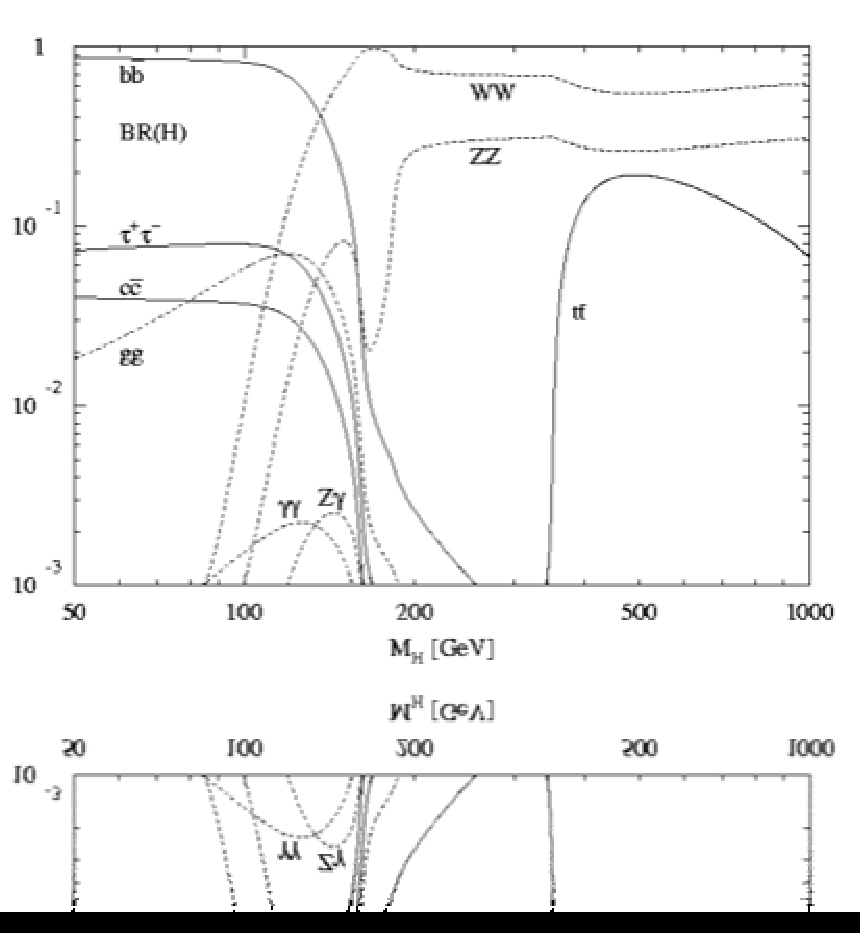
\includegraphics[trim = 0mm 45mm 0mm 0mm, clip, width=0.7\textwidth]{figs/higgs_sm_br.pdf}
%%    \caption{Standard Model Higgs branching fraction as a function of 
%%      Higgs mass}
%%    \label{figure:higgs_sm_br}}
%%\end{figure}
%%%%%%%%%
